\documentclass[11pt,a4paper]{article}

\usepackage[T1]{fontenc}
\usepackage[utf8]{inputenc}
\usepackage[provide=*,main=french]{babel}
\usepackage{lmodern}
\usepackage{microtype}
\usepackage{geometry}
\geometry{top=2.25cm,bottom=2.35cm,left=2.35cm,right=2.35cm}
\usepackage{amsmath,amssymb,amsthm,mathtools,bm}
\usepackage{graphicx}
\usepackage{booktabs,tabularx,array,multirow,longtable}
\usepackage{enumitem}
\usepackage{xcolor}
\usepackage{caption}
\usepackage{subcaption}
\usepackage{fancyhdr}
\usepackage{hyperref}
\usepackage[nameinlink,noabbrev]{cleveref}

\definecolor{deepblue}{RGB}{21,101,192}
\definecolor{deeporange}{RGB}{216,67,21}
\definecolor{deepgreen}{RGB}{46,125,50}
\definecolor{softblue}{RGB}{232,242,252}
\definecolor{softgray}{RGB}{246,247,249}
\hypersetup{
  colorlinks=true,
  linkcolor=deepblue,
  citecolor=deepblue,
  urlcolor=deeporange,
  pdftitle={Dynamiques sphériques de Transformers, volume II},
  pdfauthor={Soumission anonyme}
}

\pagestyle{fancy}
\fancyhf{}
\fancyhead[L]{Dynamiques sphériques de Transformers}
\fancyhead[R]{MLP, cycles et beaucoup de tokens}
\fancyfoot[C]{\thepage}
\setlength{\headheight}{14.3pt}
\setlength{\parindent}{0pt}
\setlength{\parskip}{0.52em}
\setlength{\emergencystretch}{3em}
\setcounter{tocdepth}{1}
\setlist{nosep,leftmargin=*}

\newtheorem{theorem}{Théorème}[section]
\newtheorem{proposition}[theorem]{Proposition}
\newtheorem{lemma}[theorem]{Lemme}
\newtheorem{corollary}[theorem]{Corollaire}
\theoremstyle{definition}
\newtheorem{definition}[theorem]{Définition}
\newtheorem{remark}[theorem]{Remarque}
\renewcommand{\proofname}{Preuve}

\newcommand{\sphere}{\mathbb S}
\newcommand{\R}{\mathbb R}
\newcommand{\T}{\mathsf T}
\newcommand{\e}{\mathrm e}
\newcommand{\norm}[1]{\left\lVert #1\right\rVert}
\newcommand{\one}{\bm 1}
\newcommand{\N}{\mathcal N}
\newcommand{\Pperp}[1]{P_{#1}^{\perp}}
\newcolumntype{Y}{>{\raggedright\arraybackslash}X}

\newenvironment{plainbox}
{\begin{center}\begin{minipage}{0.92\textwidth}\color{deepblue}\hrule\vspace{0.45em}\small\textbf{Lecture concrète.}\ \color{black}}
{\vspace{0.35em}\color{deepblue}\hrule\color{black}\end{minipage}\end{center}}

\newenvironment{resultbox}
{\begin{center}\begin{minipage}{0.92\textwidth}\color{deepgreen}\hrule\vspace{0.45em}\small\textbf{Résultat établi ici.}\ \color{black}}
{\vspace{0.35em}\color{deepgreen}\hrule\color{black}\end{minipage}\end{center}}

\newenvironment{limitbox}
{\begin{center}\begin{minipage}{0.92\textwidth}\color{deeporange}\hrule\vspace{0.45em}\small\textbf{Ce que cela ne prouve pas.}\ \color{black}}
{\vspace{0.35em}\color{deeporange}\hrule\color{black}\end{minipage}\end{center}}

\title{\textbf{Dynamiques sphériques de Transformers}\\[0.25em]
\Large Volume II : MLP, cycles continus, chaos, multi-têtes\\
et limite à beaucoup de tokens\\[0.55em]
\large Théorie et audit numérique reproductible, depuis une couche élémentaire}
\author{Soumission anonyme}
\date{Version du 16 août 2026}

\begin{document}
\maketitle

\begin{abstract}
Ce rapport part d'une couche Transformer réduite à quatre opérations : l'attention,
une connexion résiduelle, une normalisation sur la sphère, puis un MLP quadratique
suivi d'une seconde normalisation. Nous écrivons exactement tous ses points fixes et
tous ses cycles, puis nous séparons les boucles qui n'existent qu'avec des couches
fortes de celles qui survivent lorsque chaque couche devient infinitésimale. Un
recensement initial de 28 672 modèles et 2 752 512 trajectoires trouve des cycles
stables de trois et quatre couches dans les quatre familles structurelles. L'audit de
la limite faible porte finalement sur 214 528 modèles tirés indépendamment et
2 844 160 trajectoires initiales. Parmi 1 908 attracteurs complexes rejoués dans
l'équation continue, 1 699 s'arrêtent et 209 restent mobiles sur la fenêtre principale.
Le type entièrement réciproque avec MLP potentiel s'arrête dans 286 cas sur 286 ; les
trois autres types gardent des rotations, des cycles qui changent la forme des groupes,
deux attracteurs chaotiques à trois tokens et un attracteur hyperchaotique à huit
tokens. Les tests de pas, d'intégrateur, de perturbation, de divergence et de bassins
sont indépendants.

Nous étudions ensuite ce que plusieurs têtes changent : elles ne superposent pas
simplement leurs cartes de destinations, car leurs poussées s'additionnent avant que
la destination soit choisie. En grande dimension, les tokens et les forces des têtes
deviennent presque perpendiculaires, mais l'attention ne s'éteint pas : à température
fixe, elle devient souvent plus uniforme. Quand le nombre de tokens tend vers
l'infini, la somme devient une intégrale et les polygones deviennent des masses
concentrées en plusieurs positions. Enfin, nous montrons comment un MLP entraîné peut
maintenir un équilibre pendant presque toute la profondeur puis le quitter près de la
sortie, comment une première étape de Muon diffère d'une étape de gradient, et comment
des poids d'attention évoluant lentement selon un processus d'Ornstein--Uhlenbeck
créent un régime de suivi retardé. Toutes les affirmations sont classées en résultats
analytiques, observations numériques et pistes ouvertes.
\end{abstract}

\begin{plainbox}
L'attention choisit les partenaires et transporte leurs directions. Le MLP pousse
chaque token en fonction de sa propre position. Si toutes ces poussées peuvent être
résumées par une seule hauteur à gravir, les tokens finissent par s'arrêter. Si une
partie de la poussée fait réellement tourner le système, on peut obtenir une horloge,
une boucle stable ou un mouvement imprévisible. Le rapport mesure exactement où cette
circulation apparaît et si elle survit à des couches arbitrairement faibles.
\end{plainbox}

\clearpage
\tableofcontents
\newpage

\section{Réponse courte et statut des conclusions}

Le volume I du dossier traite l'attention sans MLP. Il donne la condition exacte de
tous les équilibres, la réduction spectrale lorsque $Q^{\T}K=V=V^{\T}$, les formes
polygonales et un cycle stable produit par l'attention seule lorsque score et valeur
sont déliés. Le présent volume ajoute le MLP, plusieurs têtes, beaucoup de tokens et
des poids variables avec la profondeur.

Les conclusions qui résistent à tous nos contrôles sont les suivantes.

\begin{enumerate}
  \item Un MLP placé \emph{après} l'attention change fortement une couche finie. En
  revanche, quand chaque couche devient faible, le bloc en série et un bloc où les
  deux poussées seraient additionnées ont la même équation au premier ordre ; leur
  différence commence à l'ordre $h^2$.
  \item Les quatre familles testées possèdent beaucoup de points fixes et des cycles
  stables de trois ou quatre couches. Cela ne signifie pas que ces petits cycles
  survivent à la limite continue.
  \item Dans la famille entièrement réciproque, tous les attracteurs complexes
  sélectionnés deviennent des points fixes quand on affaiblit les couches. Dès qu'un
  MLP général ou un transport de valeur non réciproque est autorisé, des mouvements
  continus peuvent survivre.
  \item Plusieurs têtes choisissent une destination par leur somme. Elles peuvent
  créer une destination absente de chaque tête prise séparément, ou couper un bassin
  en plusieurs morceaux.
  \item L'orthogonalité en grande dimension ne découple pas automatiquement les
  tokens. Avec les normalisations de notre audit, les scores deviennent proches et
  l'attention tend vers la moyenne globale.
  \item Dans la limite de beaucoup de tokens, les mêmes équations deviennent une
  équation de transport pour une distribution. Les polygones ne disparaissent pas :
  leurs nombres de tokens par sommet deviennent des proportions de masse.
  \item L'entraînement du MLP peut sélectionner quand quitter un attracteur. Notre
  expérience reproduit un long plateau suivi d'une action terminale, mais ne démontre
  pas qu'un Transformer résout arbitrairement un problème difficile.
\end{enumerate}

\begin{limitbox}
Le recensement est massif mais fini. Il ne constitue pas une preuve couvrant toutes les
matrices réelles. Nous n'affirmons ni qu'un problème NP-complet devient facile, ni
qu'une analyse par répliques est déjà établie pour ce bloc exact, ni qu'un MLP
quadratique permet d'imposer n'importe quelle configuration sans contrainte. Ces trois
idées restent des programmes de recherche.
\end{limitbox}

\section{Le bloc étudié, sans rien supposer au départ}
\label{sec:model}

\subsection{Les tokens et l'attention}

Il y a $n$ tokens. Chaque token est un vecteur $x_i\in\R^d$ de norme un. Les deux
matrices effectivement visibles par une tête d'attention sont
\[
 S=Q^{\T}K,\qquad V.
\]
$S$ décide qui regarde qui ; $V$ décide ce qui est transporté. La dynamique gelée ne
voit jamais $Q$ et $K$ séparément : deux factorisations donnant le même produit $S$
produisent exactement les mêmes trajectoires.

Pour une netteté $\beta\ge0$, posons
\begin{align}
 a_{ij}(X)&=\frac{\exp(\beta x_i^{\T}Sx_j)}
 {\sum_{k=1}^n\exp(\beta x_i^{\T}Sx_k)},\label{eq:weights}\\
 A_i(X)&=\sum_{j=1}^n a_{ij}(X)Vx_j.\label{eq:attention}
\end{align}
Même lorsque $\beta=0$, l'attention n'est pas retirée : chaque poids vaut $1/n$ et la
matrice $V$ transporte encore la moyenne des tokens.

\subsection{Le MLP quadratique}

Le plus petit MLP qui produit déjà plusieurs puits et de la circulation est
\begin{equation}
 M(x)=b+Lx+\sum_{r=1}^{m}o_r\,(u_r^{\T}x+c_r)^2.\label{eq:general-mlp}
\end{equation}
Sa largeur est $m$. Le vecteur $u_r$ décide ce que le neurone caché mesure et $o_r$
décide dans quelle direction sa réponse pousse.

Nous appelons ce MLP \emph{potentiel} lorsque
\begin{equation}
 L=L^{\T},\qquad o_r=\gamma_r u_r.\label{eq:potential-constraint}
\end{equation}
Dans ce cas il existe une fonction scalaire
\begin{equation}
 \phi(x)=b^{\T}x+\tfrac12x^{\T}Lx+
 \sum_r\frac{\gamma_r}{3}(u_r^{\T}x+c_r)^3
 \quad\text{telle que}\quad M=\nabla\phi.\label{eq:mlp-potential}
\end{equation}
Cette contrainte ne signifie pas que le MLP est faible : il peut créer plusieurs
puits. Elle interdit seulement une poussée qui tourne sans être le versant d'une même
surface.

\subsection{La vraie couche en série}

Notons $\N(z)=z/\norm z$. Une couche de force $h>0$ est
\begin{equation}
 y_i=\N\!\left(x_i+hA_i(X)\right),\qquad
 F_i(X)=\N\!\left(y_i+hM(y_i)\right).\label{eq:serial-layer}
\end{equation}
Le MLP est donc bien \emph{après} l'attention, comme dans le bloc sériel demandé. Le
modèle de contrôle d'Isobe, Inoue et Imaizumi additionne au contraire un champ FFN au
champ d'attention dans une équation continue \cite{isobe2026training}. Cette
différence architecturale est importante à pas fini ; la prochaine section précise ce
qu'elle devient lorsque $h$ tend vers zéro.

\section{Toutes les destinations et toutes les boucles}
\label{sec:exact-equations}

\subsection{Équation exacte d'un point fixe}

\begin{proposition}[Condition nécessaire et suffisante pour une couche finie]
Une configuration $X$ est un point fixe de la couche \eqref{eq:serial-layer} si et
seulement s'il existe, pour chaque token, un point intermédiaire unitaire $y_i$ et deux
nombres strictement positifs $r_i,s_i$ tels que
\begin{equation}
 x_i+hA_i(X)=r_i y_i,\qquad
 y_i+hM(y_i)=s_i x_i.\label{eq:finite-fixed}
\end{equation}
\end{proposition}

\begin{proof}
La première égalité dit exactement que la première normalisation produit $y_i$ ; la
seconde dit que la deuxième normalisation ramène vers $x_i$. La positivité de $r_i$ et
$s_i$ conserve la direction au lieu de la renverser. Réciproquement, normaliser les
deux égalités redonne \eqref{eq:serial-layer} puis $F_i(X)=x_i$.
\end{proof}

Cette écriture garde l'exponentielle du softmax dans $A_i$ mais supprime les divisions
de normalisation. Elle est donc directement utilisable par un solveur d'équations.

\subsection{Équation exacte d'un cycle de longueur quelconque}

Pour une période $p$, on introduit $X^0,\ldots,X^{p-1}$ et $Y^0,\ldots,Y^{p-1}$. On
écrit \eqref{eq:finite-fixed} à chaque étape en remplaçant le dernier $X$ par l'état
suivant, puis on ferme la boucle :
\begin{align}
 x_i^k+hA_i(X^k)&=r_i^k y_i^k,\\
 y_i^k+hM(y_i^k)&=s_i^k x_i^{k+1},\\
 X^p&=X^0.\label{eq:all-cycles}
\end{align}
Pour demander une période primitive, on exclut les retours avant $p$. Ces équations
couvrent donc tous les cycles, pas uniquement les triangles ou quadrilatères visibles.

\subsection{Équation continue et condition finale}

Pour un vecteur unitaire $x$ et une poussée $z$,
\[
 \N(x+hz)=x+h(I-xx^{\T})z+O(h^2).
\]
Appliquée deux fois à \eqref{eq:serial-layer}, cette identité donne
\begin{equation}
 \boxed{\quad\dot x_i=(I-x_ix_i^{\T})\{A_i(X)+M(x_i)\}.\quad}\label{eq:continuous}
\end{equation}
Le caractère sériel apparaît seulement dans le terme d'ordre $h^2$. Tous les
équilibres continus sont donc exactement les solutions de
\begin{equation}
 \boxed{\quad(I-x_ix_i^{\T})\{A_i(X)+M(x_i)\}=0,
 \qquad i=1,\ldots,n.\quad}\label{eq:continuous-equilibrium}
\end{equation}

\begin{plainbox}
À l'arrêt, la poussée totale peut être non nulle. Elle doit seulement être parallèle au
token. La normalisation efface alors cette partie radiale. Avec le MLP, l'attention et
le MLP peuvent aussi se neutraliser le long de la sphère : aucun des deux n'a besoin
d'être séparément à l'équilibre.
\end{plainbox}

\subsection{Stabilité}

La stabilité d'un point fixe se décide en perturbant tous les tokens dans les
directions tangentes à leur sphère. Pour une couche finie, on calcule la matrice des
dérivées de $F$ restreinte à ces directions. Le point attire si toutes ses valeurs
propres ont un module inférieur à un. Dans le flot continu, on dérive le membre droit
de \eqref{eq:continuous}. Le point attire si toutes les parties réelles sont négatives.
Ce test inclut les perturbations qui séparent deux tokens momentanément égaux ; il
évite de confondre une égalité maintenue par l'arrondi numérique avec un vrai groupe
stable.

\section{Quatre familles et inventaire à pas fini}
\label{sec:taxonomy}

Les quatre familles croisent deux choix pour l'attention et deux choix pour le MLP.

\begin{center}
\begin{tabularx}{0.9\textwidth}{cYY}
\toprule
Type & Attention & MLP \\
\midrule
1 & $S=V=V^{\T}$ & potentiel \\
2 & $S=V=V^{\T}$ & quadratique général \\
3 & $S$ et $V$ déliés & potentiel \\
4 & $S$ et $V$ déliés & quadratique général \\
\bottomrule
\end{tabularx}
\end{center}

Pour les types 3 et 4, nous avons séparé quatre sous-cas : $S$ et $V$ symétriques,
$S$ symétrique et $V$ générale, $S$ générale et $V$ symétrique, puis les deux
générales. Les largeurs MLP sont 1, 2, 4 et 8 ; le nombre de tokens va de 1 à 4 dans
l'inventaire principal.

Le premier balayage large contient 28 672 modèles, 96 départs par modèle et donc
2 752 512 trajectoires. Il teste cinq régimes de pas, de netteté et de rapport entre la
force de l'attention et celle du MLP. Le type 3 est sur-échantillonné. Il s'agit d'un
inventaire dense sur la grille choisie, pas d'une énumération de l'espace continu des
matrices.

\subsection{Beaucoup de destinations stables}

La résolution directe des équations trouve, en moyenne, les nombres suivants de
points fixes stables.

\begin{center}
\begin{tabular}{c@{\quad}ccc@{\qquad}c}
\toprule
Type & 1 token & 2 tokens & 3 tokens & maximum observé \\
\midrule
1 & 1,68 & 2,34 & 3,09 & 8 \\
2 & 1,49 & 2,03 & 2,55 & 9 \\
3 & 1,57 & 2,13 & 2,61 & 8 \\
4 & 1,31 & 1,71 & 2,00 & 7 \\
\bottomrule
\end{tabular}
\end{center}

Un contrôle construit avec trois puits donne exactement $3^n$ destinations stables
étiquetées : 3, 9, 27, 81 et 243 pour un à cinq tokens. Cela montre comment une règle
locale très simple peut créer un nombre combinatoire de répartitions finales.

\subsection{Cycles de trois et quatre couches}

Chaque candidat a été raffiné en résolvant $F^3(X)=X$ ou $F^4(X)=X$, puis son retour
primitif et sa stabilité ont été testés sur tout le cycle.

\begin{center}
\begin{tabular}{crrrr}
\toprule
Type & trajectoires p3 & modèles p3 & trajectoires p4 & modèles p4 \\
\midrule
1 & 321 & 8 & 201 & 15 \\
2 & 2 039 & 34 & 1 823 & 28 \\
3 & 4 490 & 75 & 4 507 & 113 \\
4 & 1 621 & 22 & 1 860 & 41 \\
\bottomrule
\end{tabular}
\end{center}

Des périodes primitives 5 à 12 sont également certifiées. Les quatre largeurs MLP en
contiennent. Une attention uniforme ($\beta=0$) en contient aussi. Le MLP général peut
produire seul des p3 et p4 ; le MLP potentiel seul n'a produit aucun p3 certifié dans
65 536 trajectoires, et son unique candidat p4 s'est réduit à une période plus courte.

\begin{figure}[t]
\centering
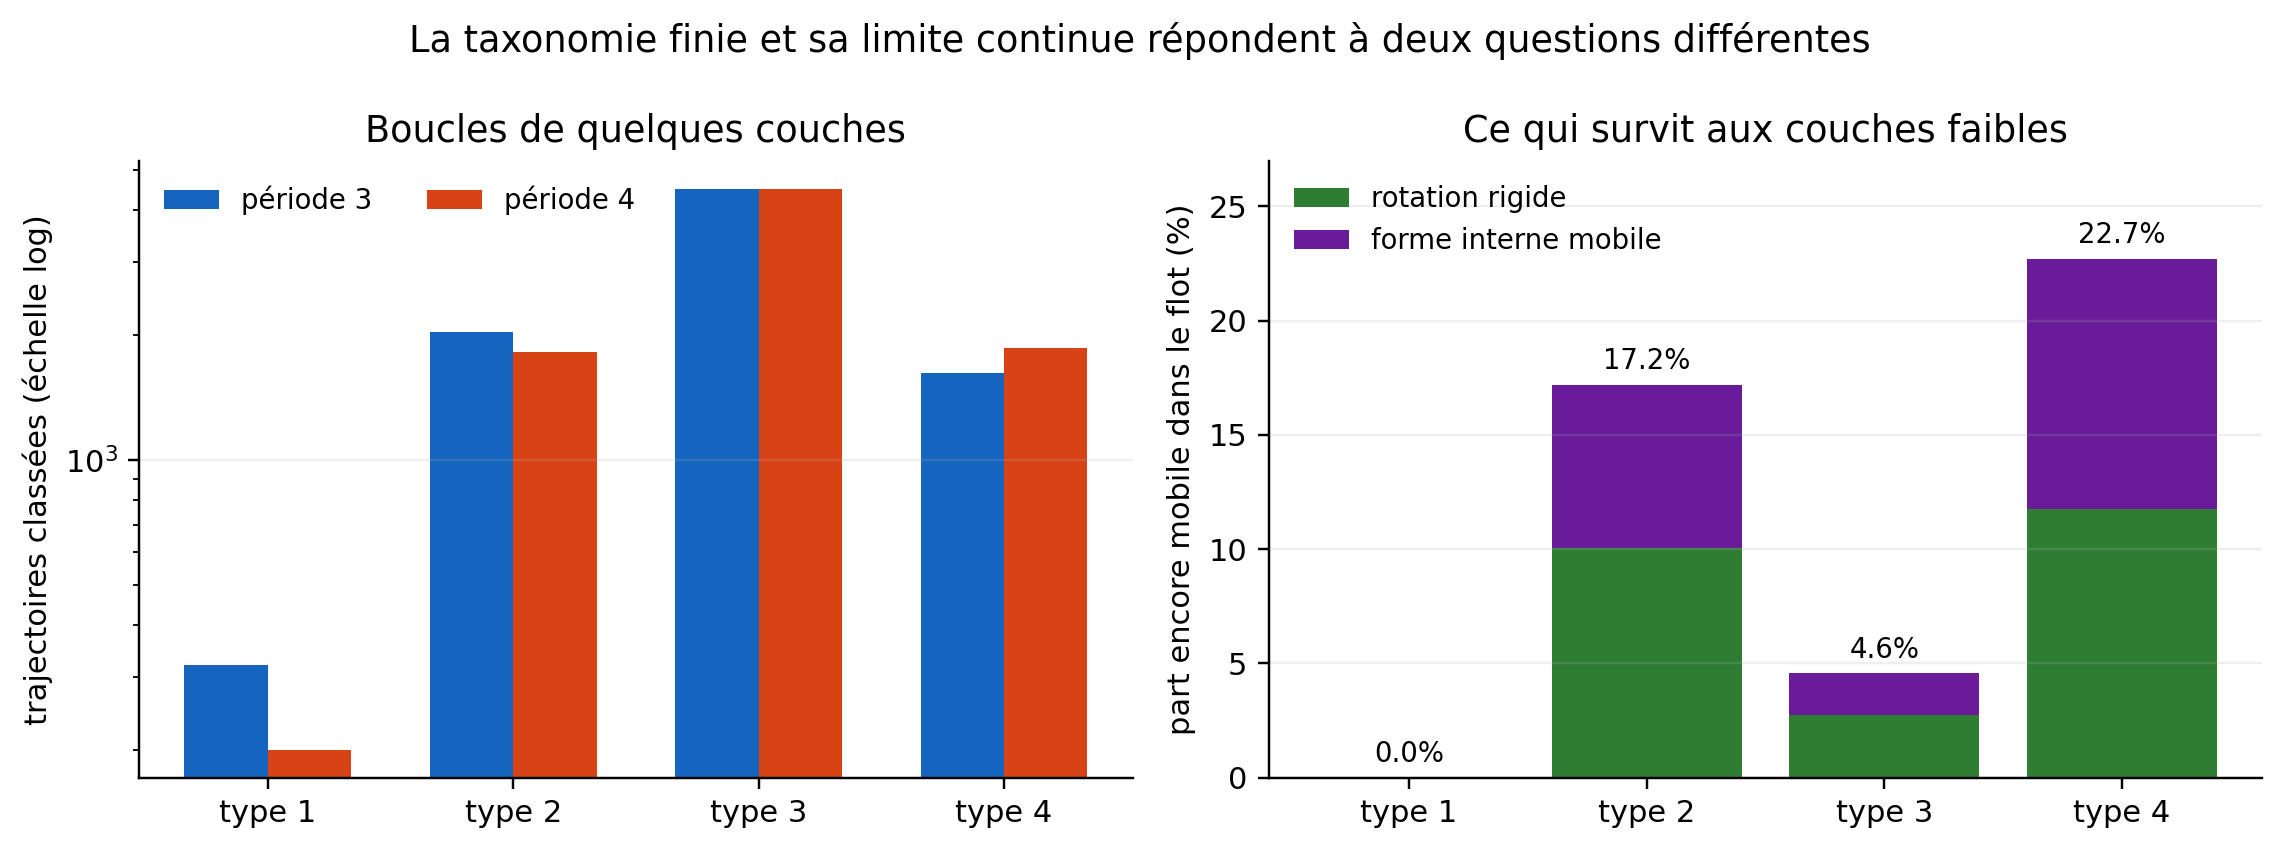
\includegraphics[width=\textwidth]{figures/taxonomy_and_survival.png}
\caption{À gauche, cycles de quelques couches dans le premier balayage. À droite,
part des attracteurs sélectionnés qui reste mobile après passage à l'équation
continue. Les deux panneaux n'ont ni le même dénominateur ni la même question.}
\label{fig:taxonomy-survival}
\end{figure}

\begin{resultbox}
La séparation décisive n'est pas simplement « potentiel ou non ». À pas fini, la
composition de deux sous-étapes peut créer une boucle même si chacune possède une
interprétation énergétique. À pas infinitésimal, ce qui compte est l'existence d'une
circulation dans la somme des deux champs.
\end{resultbox}

\section{Pourquoi les petits cycles ne suffisent pas}
\label{sec:small-step}

Supposons $F_h=I+hf+O(h^2)$. Pour une période entière $p$ fixée,
\begin{equation}
 F_h^p(x)=x+phf(x)+O(h^2).\label{eq:fixed-period-collapse}
\end{equation}
Un cycle qui garde exactement trois ou quatre couches pendant que $h$ tend vers zéro
ne peut donc s'accumuler que près d'un point où $f(x)=0$. Un vrai cycle continu peut
survivre, mais le nombre de couches nécessaires pour faire un tour doit croître comme
$T/h$, où $T$ est son temps physique de retour.

Sur toute durée physique fixée, la couche en série vérifie
\begin{equation}
 \max_{0\le k\le T/h}\norm{F_h^k(X)-\varphi_{kh}(X)}=O(h),\label{eq:finite-time}
\end{equation}
où $\varphi_t$ est le flot de \eqref{eq:continuous}. Cette convergence ne garantit pas
que deux trajectoires chaotiques restent proches pour toujours. Elle garantit que
l'équation continue est la bonne limite sur chaque fenêtre de temps fixée. Les
distributions de trajectoires et les bassins sont donc vérifiés séparément.

\subsection{Échelle finale de l'audit}

L'audit complet rassemble :

\begin{itemize}
  \item 214 528 modèles tirés indépendamment et 2 844 160 trajectoires initiales ;
  \item 26 112 contrôles frais, non sélectionnés, dans les 24 cases obtenues en croisant
  les quatre types avec 1, 2, 3, 4, 8 et 16 tokens ;
  \item 23 789 394 642 mises à jour modèle--couche, soit 102 108 101 290 mises à jour
  token--couche ;
  \item 307 200 000 évaluations RK4 de référence, soit 1 740 800 000 évaluations
  token--champ ;
  \item des pas allant jusqu'à $h/4096$, deux grilles non dyadiques, des temps physiques
  2, 10 et 20, et des contrôles de Richardson qui annulent l'erreur du premier ordre.
\end{itemize}

La pente de l'erreur est $1$ dans chaque famille. Après annulation de Richardson, elle
est $2{,}018$ sur la population principale. Au pas le plus fin, l'erreur médiane passe
de $2{,}63\times10^{-4}$ à $3{,}39\times10^{-7}$. Ce test vérifie directement le
développement $F_h=I+hf+h^2g+\cdots$.

\subsection{Recensement direct de la limite continue}

Les 1 908 attracteurs sélectionnés sont rejoués directement avec
\eqref{eq:continuous}.

\begin{center}
\begin{tabular}{crrrrr}
\toprule
Type & rejoués & fixes & mobiles & rotation rigide & forme interne mobile \\
\midrule
1 & 286 & 286 & 0 & 0 & 0 \\
2 & 378 & 313 & 65 & 38 & 27 \\
3 & 768 & 732 & 36 & 21 & 15 \\
4 & 476 & 368 & 108 & 55 & 53 \\
\midrule
Total & 1 908 & 1 699 & 209 & 114 & 95 \\
\bottomrule
\end{tabular}
\end{center}

Ainsi, 89,0\% des attracteurs complexes sélectionnés à pas fini deviennent des points
fixes ; 11,0\% restent mobiles sur la fenêtre principale. Ce taux est conditionnel à
la sélection d'un attracteur complexe : ce n'est pas sa fréquence parmi toutes les
matrices aléatoires.

Pour 8 et 16 tokens, 581 candidats sont poursuivis. Au pas $h/4096$, le comptage brut
donne 118 mouvements. Quatre états apparemment fixes ont une direction instable masquée
par des tokens numériquement égaux ; après correction, la carte finie et le flot
continu donnent tous deux 122 mouvements et s'accordent individuellement dans
575 cas sur 581. Les six différences restantes choisissent des bassins coexistants.

\section{Les mouvements continus effectivement trouvés}
\label{sec:attractors}

\subsection{Cycles stables}

Quatre cycles complets sont certifiés dans le bloc avec MLP : un p3 et un p4 issus du
type 2, puis un p3 et un p4 issus du type 4. Leur temps de retour mesuré par la carte au
pas le plus fin coïncide avec RK4 : respectivement 16,632 contre 16,660 ; 9,331 contre
9,340 ; 9,389 contre 9,400 ; 6,4395 contre 6,4400. Sur des grilles de pas qui ne sont
pas des puissances de deux, les pentes du nombre de couches par tour sont 1,0016,
1,0029, 0,9992 et 0,9950. Chaque boucle attire toutes les perturbations de son audit de
robustesse.

Le type 4 p3 est particulièrement instructif : l'attention seule garde le cycle, tandis
que le MLP seul s'arrête. Ce cas appartient donc aussi au volume I. Dans les trois
autres exemples, le MLP participe à la boucle.

\subsection{Chaos à trois tokens}

Un mouvement est appelé chaotique ici seulement après quatre contrôles : une direction
de perturbation grandit en moyenne, une direction reste neutre parce qu'elle suit le
temps le long de la trajectoire, les autres directions contractent, et la somme des
taux coïncide avec la divergence moyenne calculée indépendamment.

Le cas type 4 à trois tokens a les taux
\[
 (0{,}1489,\ 0{,}0007,\ -0{,}3923).
\]
Il reste positif dans 24 perturbations sur 24, pour trois pas RK4 ; au pas 0,005 son
premier taux vaut 0,1584. Les 512 départs uniformes testés rejoignent tous un mouvement
interne à taux positif. L'attention seule s'arrête ; le MLP seul donne une rotation
régulière ; leur interaction donne le chaos.

Un second exemple de type 2 a les taux
\[
 (0{,}0333,\ -0{,}0011,\ -0{,}7253).
\]
Ici l'attention seule et le MLP seul s'arrêtent tous les deux. Sur 512 départs, 449
dépassent le seuil strict 0,03 et les 63 autres restent positifs entre 0,022 et 0,03.

\subsection{Hyperchaos et chimère à huit tokens}

Un exemple de type 4 possède trois directions indépendantes de séparation :
\[
 (0{,}1458,0{,}1455,0{,}1435,0{,}0031,-0{,}0409,
 -0{,}1871,-0{,}1872,-0{,}1896).
\]
Une réplication avec un pas deux fois plus petit conserve trois taux positifs. Pendant
ce mouvement, quatre tokens restent synchronisés ; la trajectoire alterne surtout
entre des partitions $4+4$ et $4+3+1$. C'est une chimère : une partie du groupe reste
ordonnée pendant que les phases des groupes évoluent de façon imprévisible. Les poids
d'attention varient très peu, alors que la géométrie des tokens varie fortement.

\begin{figure}[t]
\centering
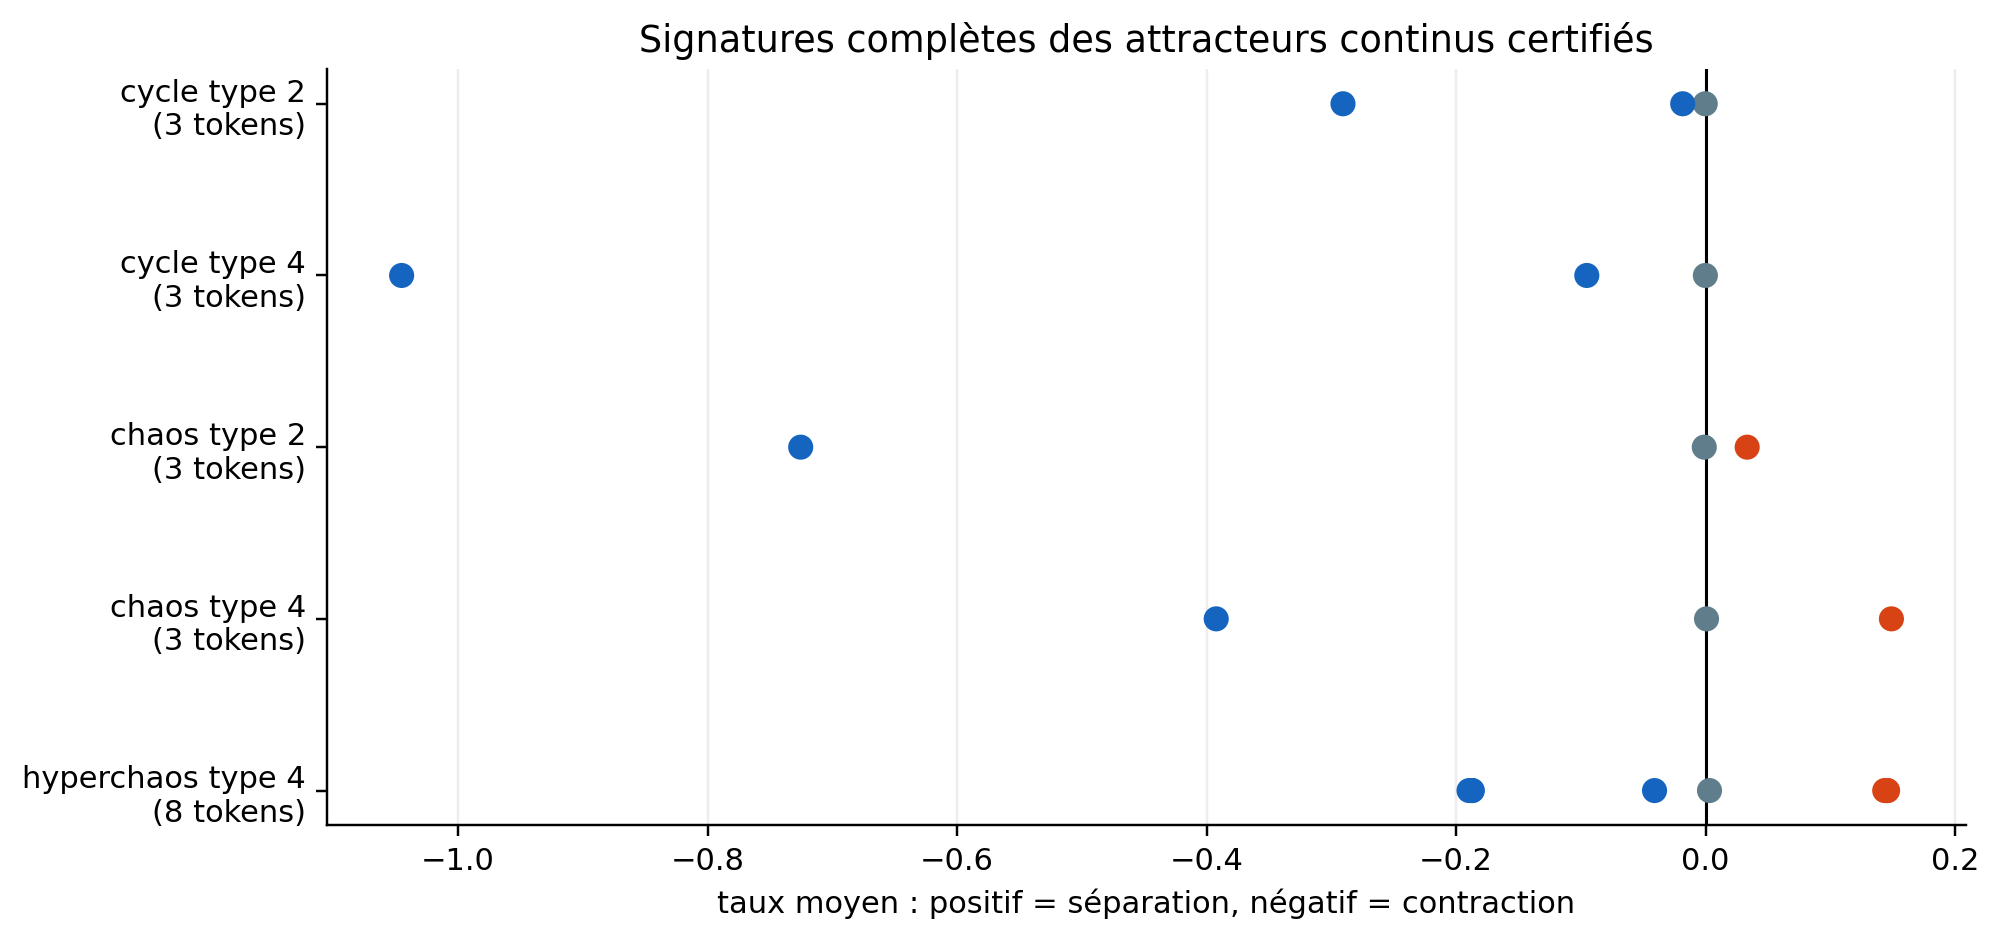
\includegraphics[width=0.92\textwidth]{figures/continuous_spectra.png}
\caption{Taux complets des cycles et attracteurs chaotiques. Un point orange à droite
de zéro signifie qu'une petite différence grandit ; un point bleu à gauche signifie
qu'elle se rétracte ; un point gris près de zéro suit la phase du mouvement.}
\label{fig:spectra}
\end{figure}

\subsection{Un cas intéressant même avec attention uniforme}

À $\beta=0$, chaque poids vaut toujours $1/n$. Pourtant un type 3 à quatre tokens
garde un mouvement intermittent avec premier taux positif. Le mécanisme vient de la
partie antisymétrique de $V$. La remplacer par sa partie symétrique, retirer l'attention
ou retirer le MLP fait converger vers un point fixe. Dans un audit de 512 départs, le
même jeu de poids possède à la fois des points fixes, des mouvements récurrents et des
trajectoires à taux positif : l'initialisation choisit le bassin.

Sur le cercle, ce cas se réécrit exactement comme un groupe d'oscillateurs couplés. La
partie antisymétrique de $V$ fournit la tendance à tourner ; le MLP potentiel fournit
des zones où le mouvement ralentit. L'attention uniforme n'est donc pas une absence
d'interaction : elle est un couplage par la moyenne globale.

\begin{limitbox}
Aucun tore quasi périodique robuste n'a encore été certifié. Nous avons certifié des
points fixes, des spirales stables, des cycles, du chaos et de l'hyperchaos, mais pas
toutes les possibilités d'un système continu de grande dimension.
\end{limitbox}

\section{Pourquoi une énergie existe parfois et parfois non}
\label{sec:energy}

Lorsque $\beta=0$, $V=V^{\T}$ et le MLP est potentiel, la fonction
\begin{equation}
 \Phi(X)=\frac{1}{2n}\sum_{i,j}x_i^{\T}Vx_j+\sum_i\phi(x_i)\label{eq:global-potential}
\end{equation}
augmente le long de la trajectoire :
\[
 \frac{d\Phi}{dt}=\sum_i\norm{(I-x_ix_i^{\T})\nabla_{x_i}\Phi}^2\ge0.
\]
Une boucle non constante reviendrait à la même valeur après un tour tout en ayant
strictement augmenté ; elle est donc impossible. Les 146 contrôles continus exacts de
ce cas finissent tous à l'équilibre.

La normalisation ligne par ligne du softmax peut briser cette structure simple même
quand $S=V=V^{\T}$. Parmi 1 699 équilibres audités, 28 sont des spirales stables : une
en type 1, dix-neuf en type 3 et huit en type 4 ; aucune n'apparaît dans le contrôle
exact $\beta=0$. La spirale isolée du type 1 montre que deux sous-champs symétriques ne
garantissent pas, avec des mobilités différentes, une seule énergie euclidienne.

En multi-têtes non normalisées, des têtes symétriques et correctement alignées
s'additionnent en une énergie commune. Avec des normalisations séparées, cette
conclusion demande des conditions supplémentaires, car chaque tête multiplie sa
poussée par son propre dénominateur. Les travaux de Pendharkar et de Massucco et
collaborateurs donnent des conditions énergétiques dans des cadres multi-têtes
précis \cite{pendharkar2026multihead,massucco2026time}. Notre audit montre ce qui se
passe lorsque les sorties ne partagent plus cette énergie.

\section{Plusieurs têtes : pas une superposition de dessins}
\label{sec:multihead}

Pour $H$ têtes, la poussée est
\begin{equation}
 A_i^{\mathrm{multi}}(X)=\sum_{h=1}^{H}\omega_h
 \sum_j a_{ij}^{(h)}(X)C_hx_j.\label{eq:multihead}
\end{equation}
La matrice de score de la tête $h$ décide ses poids ; $C_h$ inclut sa matrice de valeur
et sa recombinaison de sortie. La destination satisfait
\[
 (I-x_ix_i^{\T})\{A_i^{\mathrm{multi}}(X)+M(x_i)\}=0.
\]
Il n'est pas nécessaire que chaque tête s'annule. Deux têtes peuvent se compenser le
long de la sphère et créer une destination qui n'existe pour aucune tête seule.

\subsection{Cartes conditionnelles de bassins}

Nous fixons cinq tokens sur le cercle et laissons bouger une sixième sonde. Avec deux
matrices ayant le même spectre $(2,-3)$ mais des axes tournés de 60 degrés, la tête A
a 4 destinations, la tête B en a 5 et leur somme en a 7. Sur la sphère, les nombres
sont 4, 4 et 5. La somme coupe les frontières, déplace les destinations et crée de
petits bassins. Deux points initiaux très proches peuvent donc finir dans des groupes
éloignés s'ils sont de part et d'autre d'une frontière.

\begin{figure}[t]
\centering
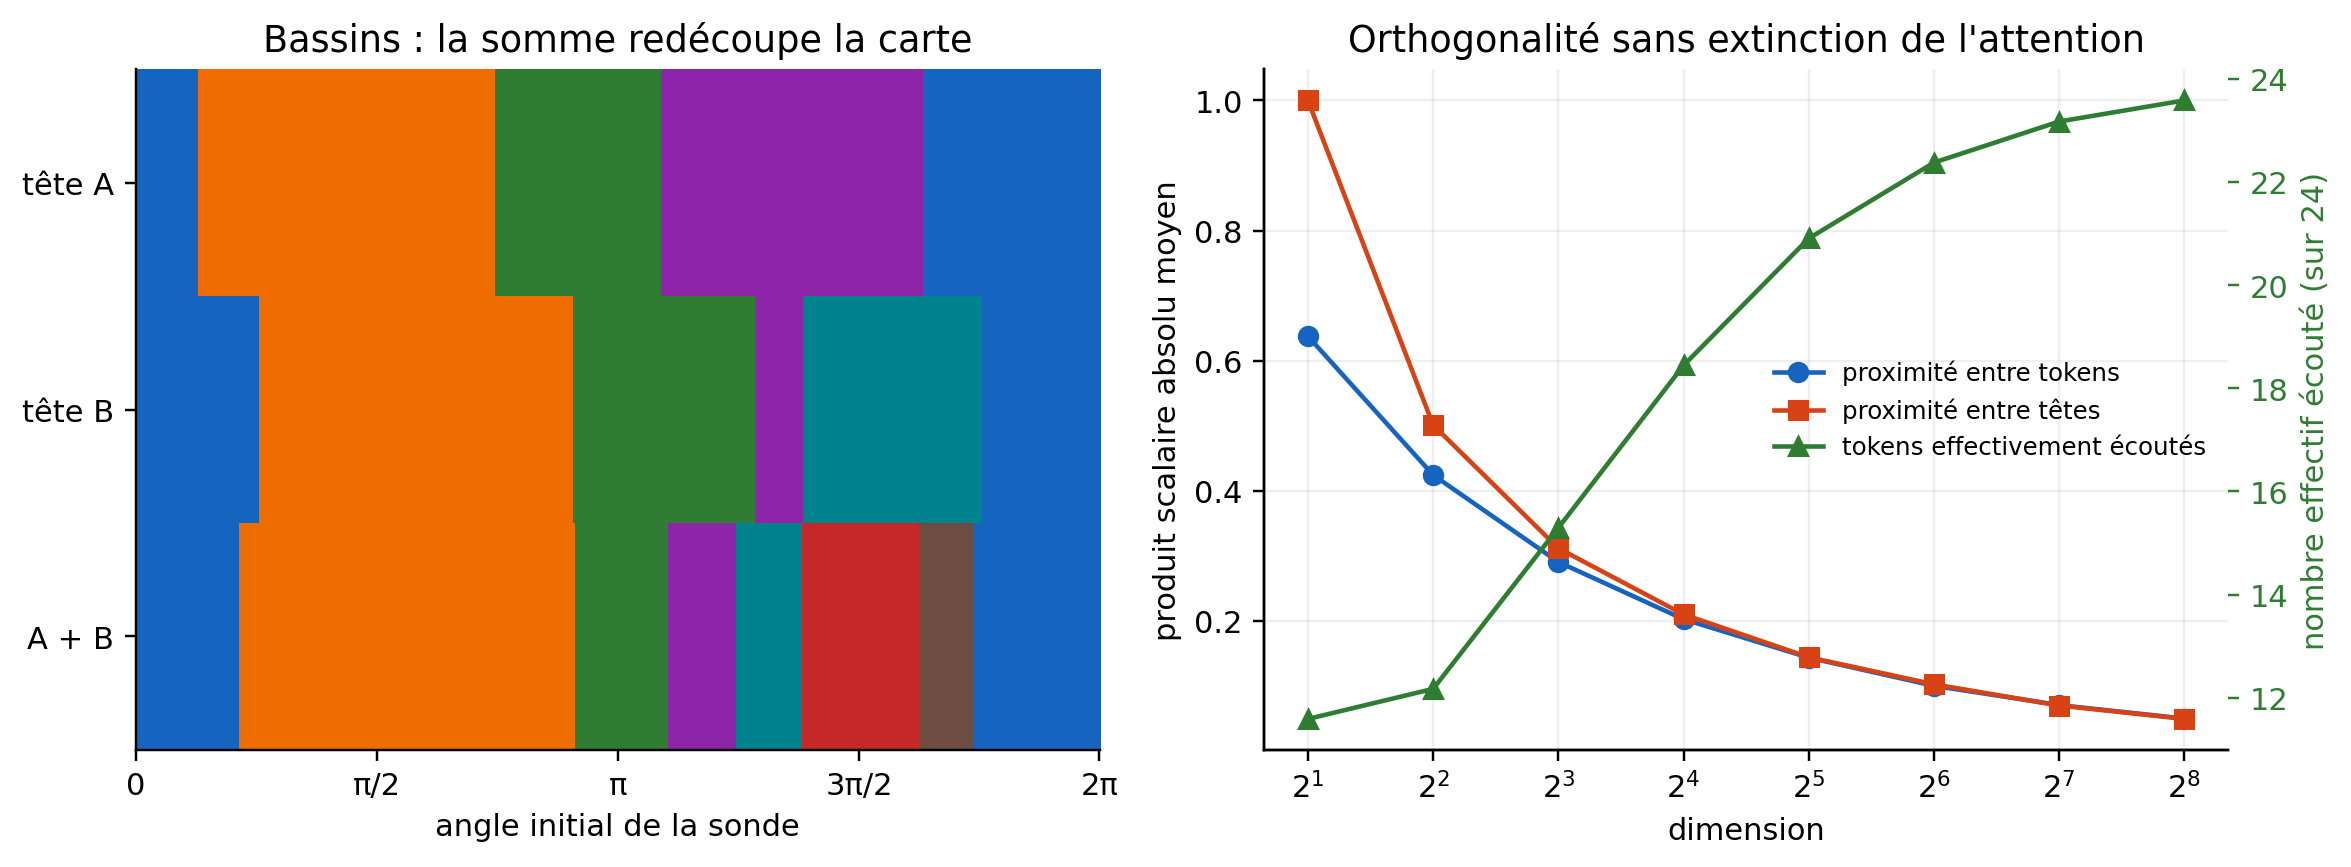
\includegraphics[width=\textwidth]{figures/multihead_and_dimension.png}
\caption{À gauche, destination de la sonde selon son angle initial : A+B n'est pas la
juxtaposition des deux premières lignes. À droite, en grande dimension, tokens et
forces deviennent presque perpendiculaires tandis que le nombre de tokens effectivement
écoutés monte vers 24.}
\label{fig:multihead-dimension}
\end{figure}

\subsection{Un cluster tournant créé par deux sorties}

Une expérience à 64 tokens utilise deux têtes avec le même score $S=I$. La première
sortie est $C_1=I$ et rassemble les tokens. La seconde est $C_2=0{,}8J$, où $J$ tourne
un vecteur de 90 degrés. Le taux de synchronisation passe de 0,471 à 1,000, mais le
cluster ne s'arrête jamais : sa vitesse angulaire mesurée vaut exactement 0,800000.
La matrice de produits scalaires reste constante pendant cette rotation. Le noyau de
score voit donc une configuration immobile alors que les valeurs transportées voient
un cycle.

\section{Grande dimension : orthogonalité sans découplage}
\label{sec:dimension}

Pour deux directions unitaires aléatoires en dimension $d$,
\[
 \mathbb E|x^{\T}y|\simeq\sqrt{\frac{2}{\pi d}}.
\]
Avec 24 tokens, six têtes aléatoires et 96 répétitions par dimension, la proximité
absolue entre tokens passe de 0,638 en dimension 2 à 0,050 en dimension 256. La
proximité entre les forces des têtes passe de 1,000 à 0,049. Les têtes indépendantes
se combinent donc presque comme des directions perpendiculaires.

Mais leurs scores deviennent aussi proches. Pour $\beta=3$ fixé, le nombre effectif
de tokens écoutés sur 24 passe de 11,6 à 23,6. La dynamique ne se décompose pas en 24
systèmes indépendants : elle conserve une moyenne globale presque uniforme.

Si $V=I$, le score propre reste 1 tandis que les scores croisés tendent vers zéro. Le
poids propre limite vaut alors
\begin{equation}
 a_{ii}\longrightarrow\frac{\e^{\beta}}{\e^{\beta}+n-1}.\label{eq:self-mass}
\end{equation}
Il faut donc $\beta$ sensiblement plus grand que $\log n$ pour un vrai auto-découplage.
Pour une matrice aléatoire sans avantage diagonal, conserver des scores non triviaux
dans notre normalisation demande typiquement $\beta$ de l'ordre de $\sqrt d$.

Dans un Transformer pratique, la division par $\sqrt{d_{\mathrm{head}}}$ et les normes
apprises des requêtes et des clés sont précisément choisies pour garder des logits
d'ordre un. L'orthogonalité brute des embeddings ne suffit donc pas à prédire le
découplage d'un réseau entraîné.

\section{Quand les tokens deviennent une distribution}
\label{sec:meanfield}

Définissons la mesure empirique
\[
 \mu_t^n=\frac1n\sum_{i=1}^n\delta_{x_i(t)}.
\]
Pour un noyau positif $g$ et une attention normalisée, la vitesse au point $x$ est
\begin{equation}
 v_g[\mu](x)=P_x^{\perp}
 \frac{\int g(x^{\T}Sy)Vy\,d\mu(y)}
 {\int g(x^{\T}Sy)\,d\mu(y)}+P_x^{\perp}M(x).\label{eq:mean-field-velocity}
\end{equation}
La limite de beaucoup de tokens est l'équation de transport
\begin{equation}
 \partial_t\mu_t+\operatorname{div}_{\sphere}
 \bigl(\mu_t v_g[\mu_t]\bigr)=0.\label{eq:transport}
\end{equation}
Elle dit seulement que toute la masse de tokens est déplacée par un champ calculé à
partir de la distribution entière. Les travaux de Rigollet et de Castin, Ablin,
Carrillo et Peyré placent cette limite dans une géométrie de transport adaptée à la
normalisation \cite{rigollet2025meanfield,castin2025unified}.

Dans notre contrôle, une densité à trois bosses est échantillonnée puis comparée à une
quadrature de 8 192 points. L'erreur sur la vitesse décroît comme $n^{-0{,}494}$, en
accord avec la fluctuation $n^{-1/2}$ : 0,289 à 16 tokens, 0,146 à 64, 0,071 à 256 et
0,038 à 1 024.

\subsection{Les polygones deviennent des masses}

Une distribution concentrée sur $q$ positions s'écrit
\[
 \mu=\sum_{a=1}^q p_a\delta_{w_a},\qquad p_a>0,\quad\sum_a p_a=1.
\]
Elle est stationnaire exactement lorsque
\begin{equation}
 P_{w_a}^{\perp}
 \sum_b p_b g(w_a^{\T}Sw_b)Vw_b+P_{w_a}^{\perp}M(w_a)=0
 \quad\text{pour chaque }a.\label{eq:atomic-equilibrium}
\end{equation}
Les nombres entiers de tokens placés à chaque sommet deviennent donc des masses
réelles. Le passage à l'intégrale élargit la famille : les rapports de masses n'ont
plus besoin d'être rationnels.

\begin{figure}[t]
\centering
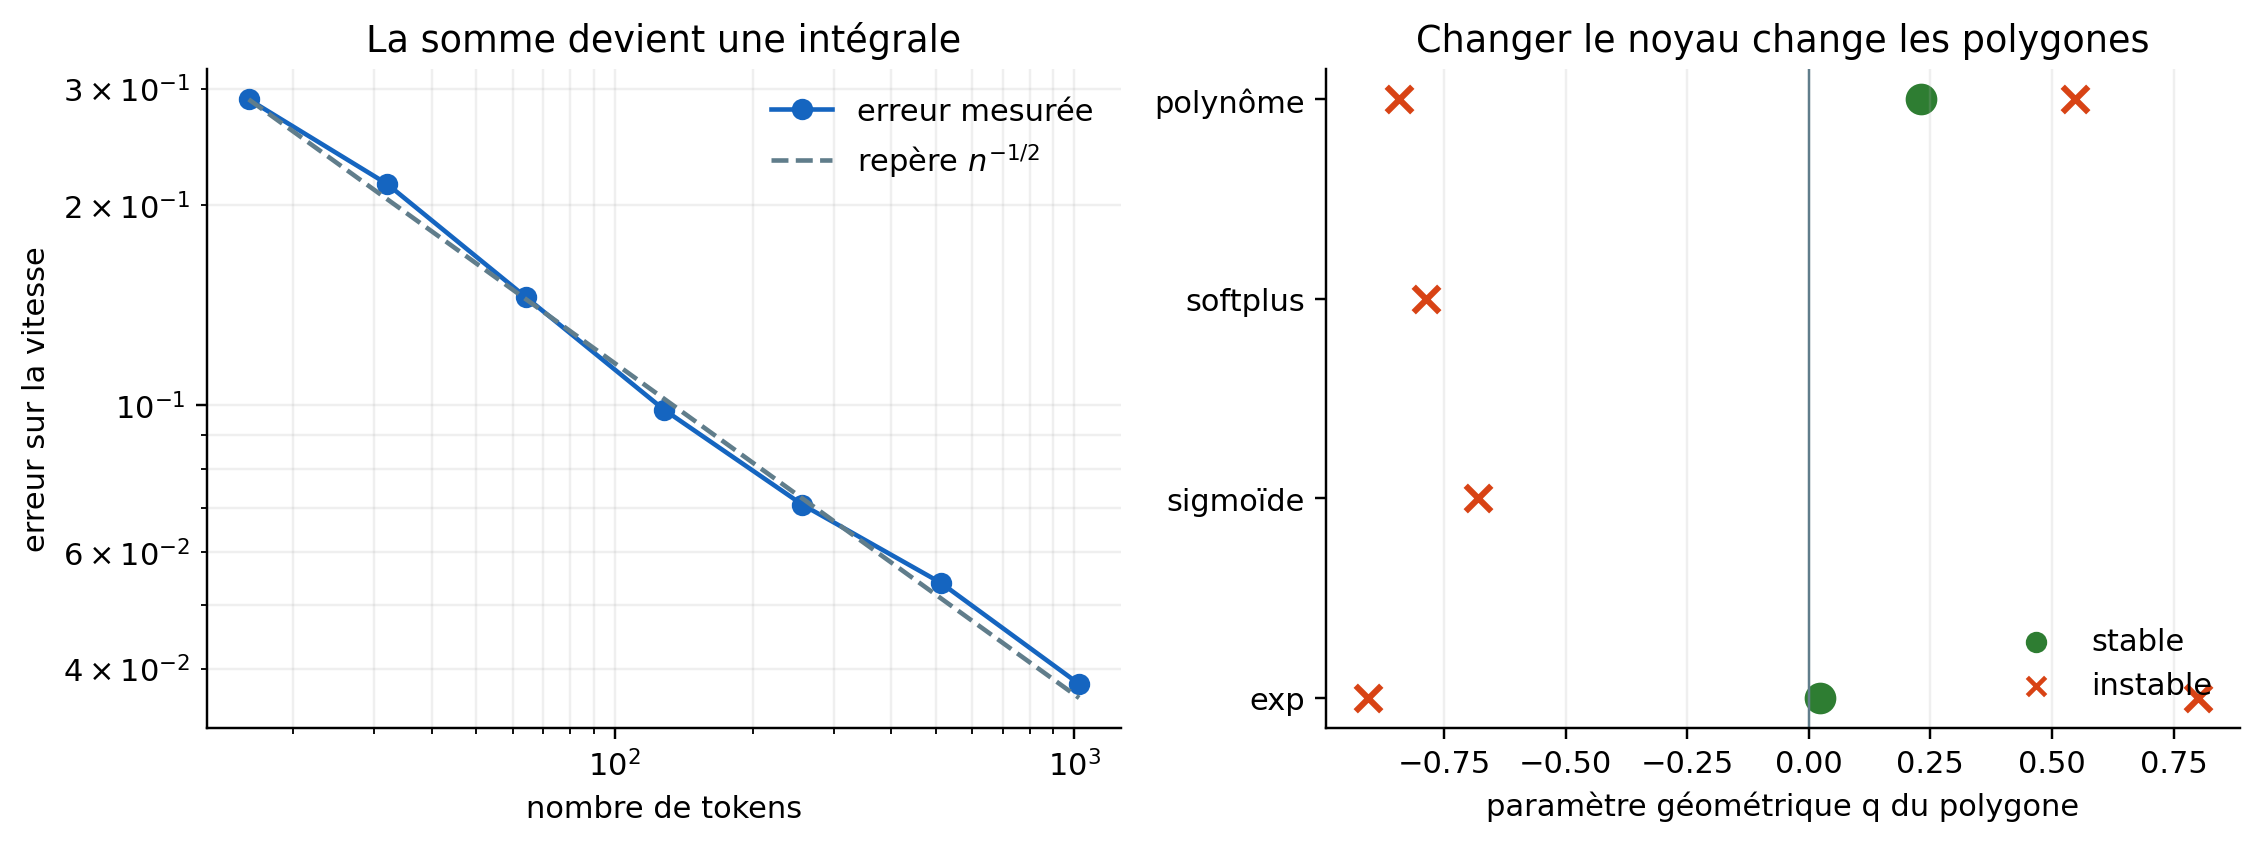
\includegraphics[width=\textwidth]{figures/meanfield_and_kernels.png}
\caption{À gauche, convergence de la somme de tokens vers l'intégrale. À droite,
positions polygonales trouvées pour quatre noyaux ; le cercle vert indique une branche
stable et la croix orange une branche instable.}
\label{fig:meanfield-kernels}
\end{figure}

\subsection{Que mesure Wasserstein ?}

La distance de Wasserstein mesure le coût minimal pour déplacer un nuage de masse vers
un autre. Elle convient naturellement à \eqref{eq:transport}. Elle ne transforme pas
automatiquement toute attention en descente d'énergie. Sans dénominateur et avec une
interaction symétrique, une primitive $G$ de $g$ donne l'énergie
\[
 \mathcal E_G(\mu)=\frac12\iint G(x^{\T}Vy)\,d\mu(x)d\mu(y).
\]
Le dénominateur du softmax change la mobilité locale. Des matrices déliées ou
antisymétriques peuvent supprimer toute énergie commune.

\section{Changer l'exponentielle ou la normalisation}
\label{sec:kernels}

Nous remplaçons $\exp(1{,}5s)$ par trois noyaux positifs dans le cas
$V=\operatorname{diag}(2,-3)$ et trois masses égales.

\begin{center}
\begin{tabularx}{0.88\textwidth}{YYl}
\toprule
Noyau & racines polygonales $q$ & racine stable \\
\midrule
exponentielle & $-0{,}907,\ 0{,}024,\ 0{,}801$ & $0{,}024$ \\
sigmoïde bornée & $-0{,}680$ & aucune \\
softplus & $-0{,}787$ & aucune \\
polynôme $(1+s/3{,}01)^4$ & $-0{,}842,\ 0{,}231,\ 0{,}548$ & $0{,}231$ \\
\bottomrule
\end{tabularx}
\end{center}

L'exponentielle n'est donc pas nécessaire à l'existence d'une forme polygonale, mais
elle change ses branches et leur stabilité. Pour un noyau positif $g$, retirer
seulement le dénominateur ne change pas les équilibres : il multiplie la vitesse par
un facteur positif. Il peut cependant changer fortement les temps, les bassins et la
métastabilité.

Retirer la sphère est une opération bien plus radicale. Un token placé sur la direction
propre positive de valeur 2 garde sa norme avec la projection sphérique. Sans cette
projection, sa norme atteint 10 au temps 1,151 avec attention normalisée ; sans sphère
ni dénominateur, elle diverge au temps 0,003262 dans notre paramétrage exponentiel. Une
poussée auparavant radiale et invisible change alors toute la dynamique.

\section{Le bon espace observable}
\label{sec:observable}

Les poids d'attention seuls ne décrivent pas l'état. Pour chaque tête, la vitesse
dépend des deux fonctions
\begin{equation}
 Z_h^{\mu}(x)=\int k_h(x,y)d\mu(y),\qquad
 N_h^{\mu}(x)=\int k_h(x,y)C_hy\,d\mu(y).\label{eq:observables}
\end{equation}
La tête utilise $N_h/Z_h$. Il faut donc observer à la fois qui est choisi et ce qui est
transporté. Avec un MLP quadratique, il faut aussi garder les mesures cachées
$u_r^{\T}x_i+c_r$ et les projections linéaires utilisées en sortie.

Pour le cas symétrique aligné, la matrice $H=XVX^{\T}$ et ses morceaux par espace
propre constituent une description fermée, à rotation près. Dans le cas général, une
description minimale utile contient :

\begin{enumerate}
  \item la géométrie des tokens, par exemple leur matrice de produits scalaires ;
  \item les matrices de score et les poids de chaque tête ;
  \item les directions après passage par les valeurs et les sorties ;
  \item les features cachées du MLP ;
  \item pour une tâche supervisée, les positions, labels et le readout.
\end{enumerate}

L'exemple hyperchaotique rend ce point mesurable : l'écart-type temporel maximal des
poids vaut seulement 0,0034, alors que celui de la géométrie de Gram vaut 0,481. Dans
l'exemple à attention uniforme, la distance entre poids est exactement zéro à tous les
pas, même lorsque la géométrie ne l'est pas.

\section{Entraîner le MLP pour choisir la sortie}
\label{sec:training}

Isobe, Inoue et Imaizumi fixent une attention symétrique non normalisée, ajoutent du
bruit et entraînent seulement un FFN linéaire en ses paramètres avec un coût
quadratique \cite{isobe2026training}. Leur solution optimale a trois phases : les
tokens se regroupent, restent longtemps près d'un puits, puis le FFN agit fortement
près de la sortie pour réduire la perte terminale. Leur attention est en parallèle
avec le FFN dans l'équation continue ; notre MLP est en série dans la couche finie.
La section \ref{sec:model} montre pourquoi le mécanisme se compare au premier ordre,
mais pas couche par couche à grand pas.

\subsection{Contrôle entraîné autour d'un polygone}

Nous entraînons un petit contrôle angulaire, linéaire en cinq features de Fourier, pour
déplacer un polygone stable vers une cible tournée de 0,9 radian. Le contrôle maximal
dans la première moitié vaut 0,0011 ; dans les cinq derniers intervalles, il atteint
2,19. L'erreur terminale vaut 0,00133. La force est donc environ 2 000 fois plus grande
à la fin qu'au début. Le plateau d'Imaizumi survit lorsque le puits n'est plus un
consensus mais un polygone.

\begin{figure}[t]
\centering
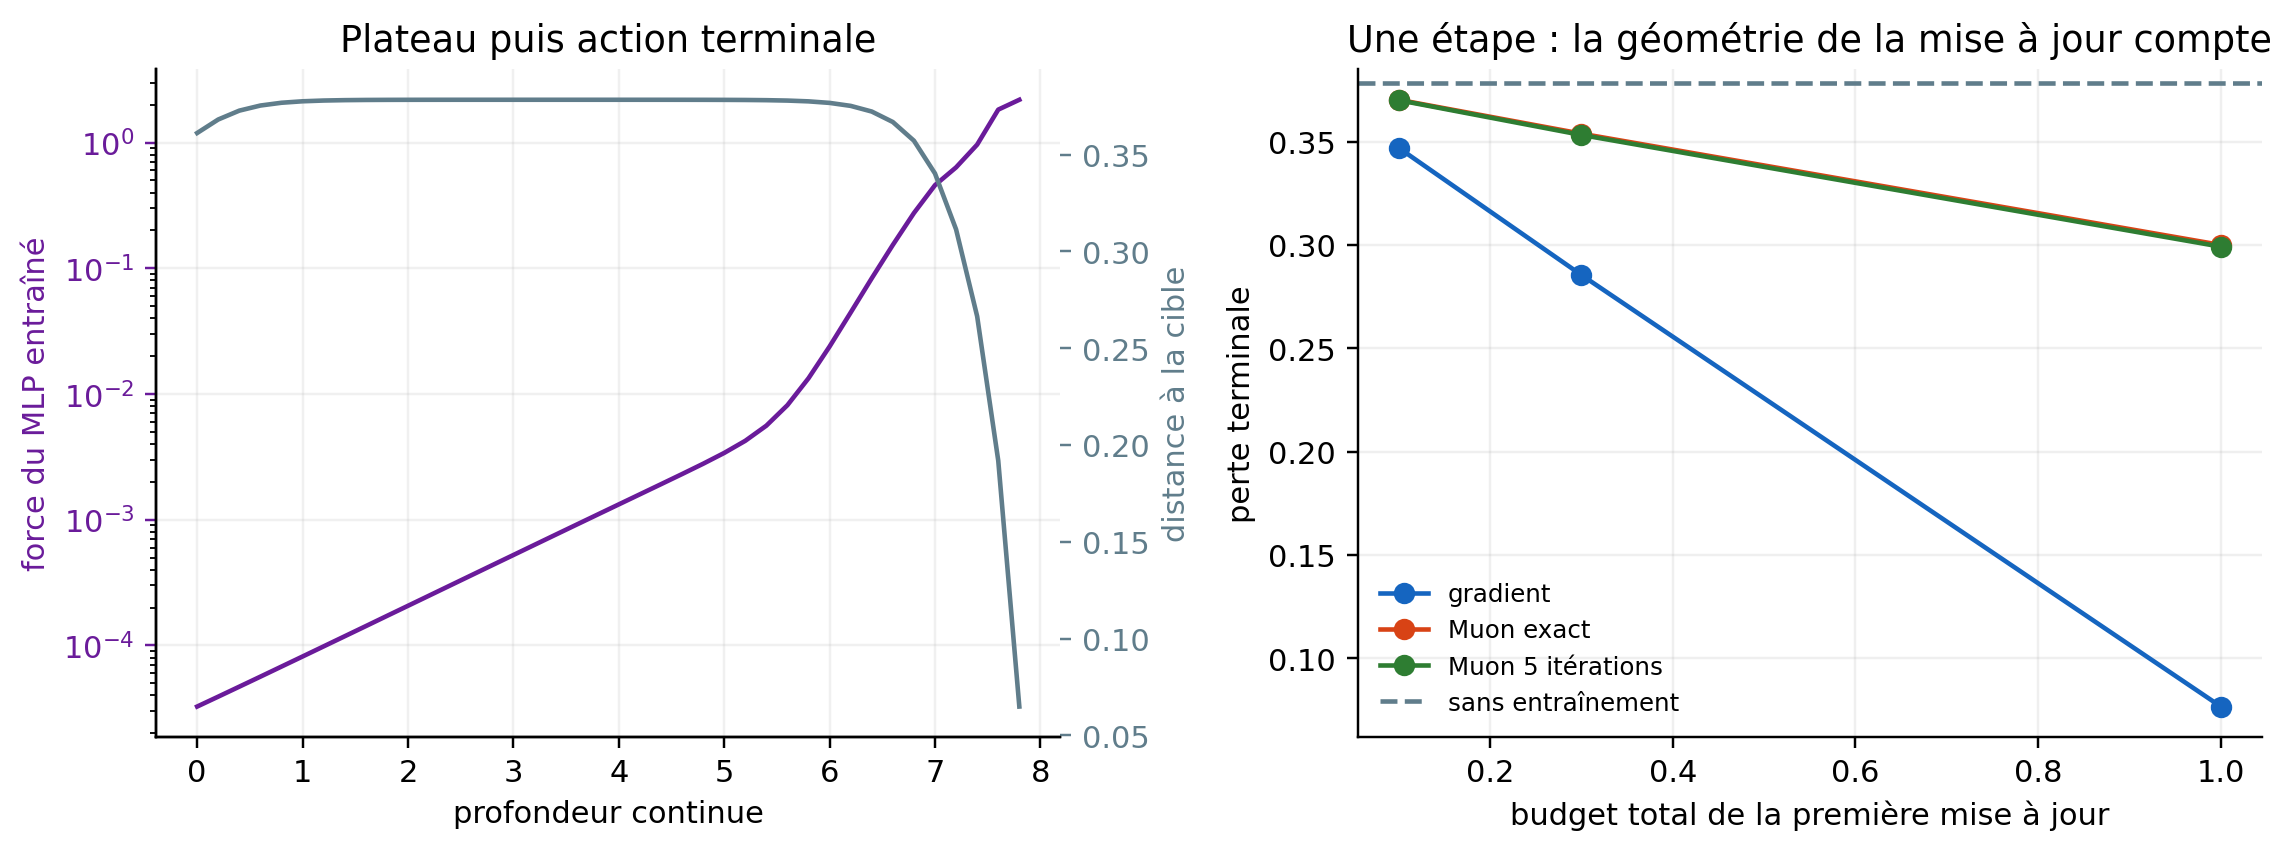
\includegraphics[width=\textwidth]{figures/training_and_muon.png}
\caption{À gauche, contrôle entraîné : le polygone absorbe d'abord les perturbations,
puis le MLP agit près de la sortie. À droite, une seule mise à jour à norme globale
égale : le gradient et Muon optimisent des géométries différentes.}
\label{fig:training-muon}
\end{figure}

Ce résultat donne un principe de conception : fixer une dynamique d'attention qui
crée des bassins utiles, puis entraîner un MLP sériel pour rester dans un bassin, en
sortir ou déplacer sa destination. Il ne garantit pas que toute condition algébrique
soit encodable par un petit MLP, ni que l'entraînement trouve globalement les bons
poids.

\subsection{Une première étape de Muon}

Si le gradient d'une matrice à la profondeur $k$ est
$G_k=U_k\Sigma_kV_k^{\T}$, une étape de gradient est $-\alpha G_k$. Une étape de Muon
idéalisée utilise plutôt
\begin{equation}
 -\eta U_kV_k^{\T}.\label{eq:muon}
\end{equation}
Elle garde les directions singulières et égalise les tailles non nulles. À la première
étape, le momentum ne change que l'échelle globale du gradient, ensuite supprimée par
ce facteur polaire. Sous une contrainte de norme opérateur par matrice, cette direction
est la plus descendante ; sous la contrainte $L^2$ du théorème d'Imaizumi, le gradient
est naturellement favorisé.

Dans notre analogue à 40 tranches, le gradient final est
$7{,}11\times10^{11}$ fois plus grand que le gradient initial. À budget total 0,3, la
perte passe de 0,37839 sans entraînement à 0,28547 avec le gradient, 0,35385 avec Muon
exact et 0,35323 avec cinq itérations de Newton--Schulz. À budget 1,0, Muon agit bien
plus tôt et détruit le plateau, tandis que le gradient concentre encore son action sur
la dernière tranche. Ce n'est pas un classement universel : il montre que la norme
choisie pour comparer les mises à jour décide du gagnant.

Des analyses récentes de mémoire associative expliquent autrement l'intérêt de Muon :
il rend l'apprentissage des directions rares plus équilibré que des mises à jour
anisotropes \cite{wang2025muon,kim2026spectral}. Notre expérience ne remplace pas ces
résultats ; elle montre leur analogue dans la profondeur d'une dynamique polygonale.

\section{Poids variables avec la profondeur : premier audit OU lent}
\label{sec:ou}

Massucco et collaborateurs représentent les têtes par une distribution de matrices qui
change avec la profondeur \cite{massucco2026time}. Dans leur régime
Ornstein--Uhlenbeck,
\begin{equation}
 dD_t=(F-D_t)dt+\sqrt{2\sigma^2}\,dW_t,\label{eq:ou}
\end{equation}
la loi des poids revient exponentiellement vers une gaussienne centrée en $F$. Leur
théorie et leurs expériences montrent alors la relaxation vers une configuration
stationnaire ; avec des poids périodiques non amortis, la relaxation peut disparaître.

Notre première approche isole la vitesse de renouvellement. Elle utilise 32 tokens sur
$\sphere^2$, quatre têtes, 12 répétitions, $\sigma=0{,}65$, un pas 0,02 et 2 000 pas.
La matrice moyenne cible a les valeurs propres $(1{,}2,1{,}0,0{,}2)$. Le taux OU varie
de 0 à 10.

\begin{figure}[t]
\centering
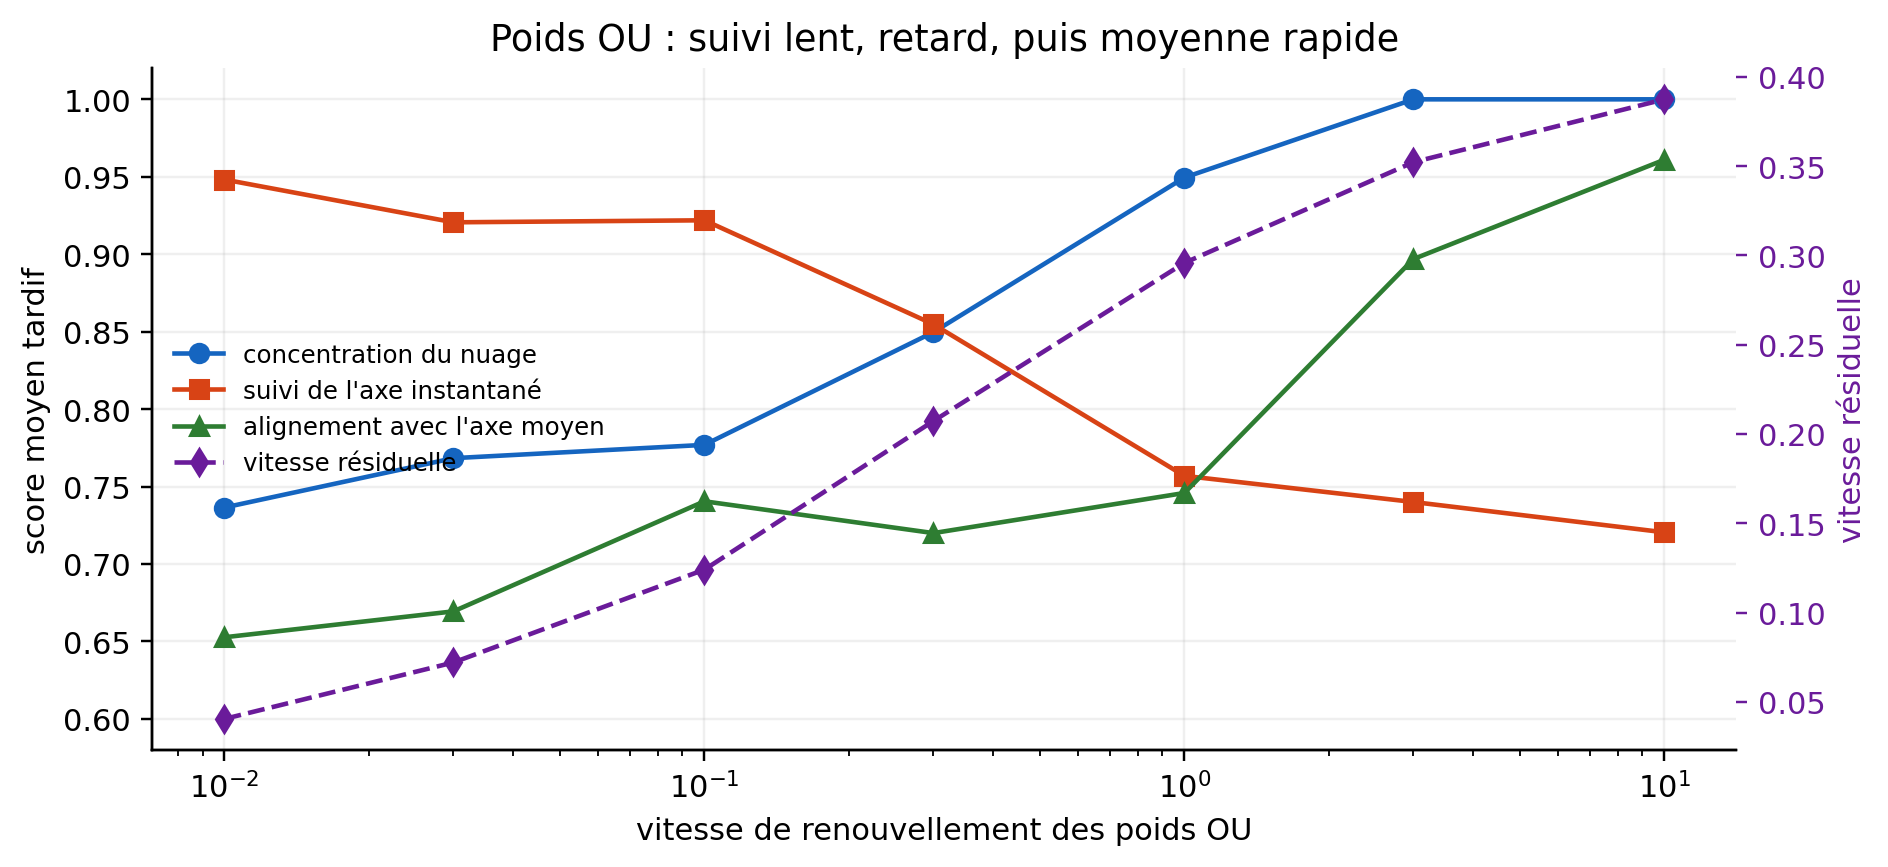
\includegraphics[width=0.88\textwidth]{figures/slow_ou.png}
\caption{Premier balayage du temps de corrélation des poids. À faible taux, le paysage
reste longtemps déformé et le nuage ne se concentre pas complètement. À taux
intermédiaire, les tokens tentent de suivre un axe mouvant avec retard. À taux élevé,
le bruit se moyenne vite, le nuage se concentre près de l'axe moyen mais garde une
vitesse instantanée élevée.}
\label{fig:slow-ou}
\end{figure}

À taux 0,01, la concentration tardive vaut 0,736 et le suivi de l'axe instantané 0,948.
À taux 0,3, elles valent 0,850 et 0,855. À taux 3, la concentration est pratiquement 1,
mais le suivi instantané n'est plus que 0,740 tandis que l'alignement avec l'axe moyen
vaut 0,897. La vitesse tardive croît de 0,040 à 0,352. Cela met en évidence trois
temps : la contraction des tokens, le mouvement du paysage et le moyennage du bruit.

\begin{plainbox}
Lent ne signifie pas nécessairement plus chaotique. Si les tokens se contractent bien
plus vite que les poids ne bougent, ils suivent quasi statiquement une branche. La
complexité apparaît près des changements de bassin et lorsque les deux temps deviennent
comparables : retard, sauts, mémoire du chemin et coexistence. Le présent balayage
mesure le retard et la concentration ; il ne certifie pas encore un attracteur
chaotique causé par l'OU lent.
\end{plainbox}

\section{Lecture de physique statistique, précisément}
\label{sec:statphys}

Chaque ligne de softmax est exactement une loi de Boltzmann conditionnelle :
\[
 a_{ij}=\frac{\e^{-E_{ij}/T}}{\sum_k\e^{-E_{ik}/T}},
 \qquad E_{ij}=-x_i^{\T}Sx_j,\qquad T=1/\beta.
\]
Cela ne fait pas encore du système une matière à l'équilibre : les poids sont des
probabilités de Boltzmann, mais la trajectoire des tokens est déterministe. Un vrai bain
thermique demanderait un bruit brownien tangent. Si le champ est un gradient et le
bruit accordé à sa mobilité, la loi stationnaire est de Gibbs. Avec transport
antisymétrique ou MLP général, des courants peuvent persister et le système reste hors
équilibre.

Les modèles voisins sont les mémoires de Hopfield modernes, les spins XY ou Heisenberg,
les oscillateurs de Kuramoto ou Lohe et les verres de spins
\cite{ramsauer2021hopfield,tiberi2024interplay}. Notre cas exact se distingue par trois
traits : le couplage dépend de l'état, il est normalisé séparément pour chaque token,
et les valeurs transportées peuvent ne pas être réciproques.

Une analyse de répliques demanderait de choisir un ensemble aléatoire précis de
matrices, une limite conjointe du nombre de tokens, de la dimension et du nombre de
têtes, puis un observable de recouvrement. La matrice des produits scalaires entre deux
copies soumises aux mêmes poids est un candidat naturel, mais les poids d'attention ne
suffisent pas : les valeurs et les features du MLP doivent aussi entrer. Les travaux de
physique statistique des chemins d'attention sont voisins, sans fournir à ce jour la
solution par répliques de notre bloc sériel exact \cite{tiberi2024interplay}.

\section{Ce qui est nouveau par rapport à Altafini et au cas symétrique}
\label{sec:new}

Altafini étudie une dynamique d'attention et sa multistabilité sans MLP sériel ; son
écriture travaille avec les matrices effectives de l'interaction plutôt qu'avec une
factorisation architecturale séparée $Q/K$ \cite{altafini2025multistability}. Son
résultat d'instabilité des équilibres polygonaux concerne sa classe précise, notamment
les configurations où la somme reçue s'annule. Il ne dit pas que toute forme à plusieurs
sommets, après ajout d'un MLP ou déliaison score--valeur, doit être instable.

Kuehn et Yoon imposent $Q^{\T}K=V=V^{\T}$ et obtiennent une sélection par les espaces
propres ainsi qu'une structure de flot de gradient \cite{kuehnyoon2026spectral}. Le
volume I étend l'équation des équilibres à $S\ne V$ et certifie un cycle interne stable
produit par l'attention seule. Le présent volume ajoute :

\begin{enumerate}
  \item la condition exacte de tous les points fixes et cycles du bloc sériel
  attention--MLP ;
  \item une taxonomie expérimentale des quatre croisements réciproque/délié et
  potentiel/général ;
  \item la preuve que les p3/p4 fixes ne peuvent rester des p3/p4 quand $h\to0$, puis
  leur audit jusqu'à $h/4096$ ;
  \item des cycles continus stables, deux chaos à trois tokens et un hyperchaos à huit
  tokens dans le bloc complet ;
  \item la démonstration que des poids d'attention constants peuvent cacher un
  mouvement interne ;
  \item des cartes multi-têtes où la somme crée de nouvelles destinations ;
  \item la distinction expérimentale entre orthogonalité, uniformisation et vrai
  découplage en grande dimension ;
  \item le passage des polygones finis aux mesures atomiques, le changement de noyau,
  le contrôle entraîné, une étape de Muon et le premier balayage OU lent.
\end{enumerate}

\begin{resultbox}
L'ajout central n'est pas « davantage de formes ». C'est une règle permettant de
distinguer les formes qui sont de vraies destinations, les boucles artificielles d'une
couche trop forte, et les mouvements qui restent vivants dans une profondeur continue.
Cette règle repose sur l'équation tangentielle finale, l'échelle $1/h$ du temps de
retour et le spectre complet des perturbations.
\end{resultbox}

\section{Ce que la dynamique peut réellement résoudre}
\label{sec:problems}

Les solutions exactes produites par la dynamique sont les vecteurs unitaires qui
satisfont \eqref{eq:continuous-equilibrium}, ou les suites périodiques qui satisfont
\eqref{eq:all-cycles}. En choisissant $S,V$ et $M$, on choisit donc une famille
d'équations non linéaires sur un produit de sphères. Les cas potentiels correspondent à
des conditions de stationnarité avec contraintes de norme ; les cas non potentiels
ajoutent une circulation et ne sont plus la minimisation d'une seule fonction.

Cela permet d'encoder des tâches utiles : mémoire associative, regroupement, choix
parmi plusieurs codes sphériques, maintien d'une horloge, suivi d'un paysage variable,
ou contrôle d'un état vers une cible. Cela ne rend pas automatiquement facile le
problème inverse « trouver les poids qui réalisent la bonne famille de solutions ».
L'entraînement peut lui-même rester non convexe, posséder de mauvais bassins et exiger
un nombre exponentiel d'essais.

MaxCut fournit un bon contre-exemple à une conclusion trop forte. On peut encoder des
signes unitaires et une énergie de coupe, puis laisser une dynamique chercher un point
stationnaire. Elle peut donner une excellente coupe et le bruit OU peut aider à changer
de bassin. Cela ne prouve ni l'optimalité globale ni un algorithme polynomial pour tous
les graphes. Le bon énoncé est : cette dynamique forme une nouvelle famille
d'heuristiques continues et entraînables pour des équations contraintes ; leur
complexité doit être étudiée problème par problème.

\section{Limites, contrôles manquants et expériences prioritaires}
\label{sec:limits}

Les contrôles les plus importants qui restent sont :

\begin{enumerate}
  \item reproduire les cycles et le chaos avec de vraies dimensions de tête, des
  matrices $W^O$ explicites et RMSNorm plutôt qu'une sphère idéale ;
  \item entraîner le bloc sériel complet, et pas seulement un contrôle FFN réduit, sur
  une tâche avec validation hors échantillon ;
  \item faire varier conjointement nombre de tokens, dimension, température et nombre
  de têtes afin de distinguer limite moyenne, limite de tête et limite de dimension ;
  \item cartographier les bifurcations lorsque les poids OU évoluent aussi lentement que
  le temps de relaxation des tokens, avec mesures d'hystérésis et de sauts de bassin ;
  \item tester si les attracteurs chaotiques certifiés persistent après ajout de bruit,
  de biais, de LayerNorm affine et de précision réduite ;
  \item construire une expérience de répliques avec deux copies et mêmes poids, puis
  mesurer le recouvrement complet incluant valeurs et MLP ;
  \item donner une borne d'approximation reliant la largeur et le degré du MLP aux
  champs tangentiels réalisables sur la sphère ;
  \item séparer performance d'optimisation et coût total pour Muon, gradient et Adam
  sur le même contrôle de profondeur.
\end{enumerate}

\section{Conclusion sans jargon}

Un token reçoit deux sortes de coups. L'attention lui dit vers quels autres tokens se
tourner. Le MLP lui donne une poussée qui dépend de sa propre position. Après chaque
coup, la normalisation le remet sur la sphère.

Pour savoir où tout peut finir, il suffit de vérifier une règle : après addition de
toutes les poussées, il ne doit rester aucun morceau qui fasse glisser le token le long
de la sphère. Cette règle donne toutes les destinations, même lorsqu'elles ont plusieurs
groupes et même lorsque l'attention et le MLP se compensent.

Les boucles demandent plus de prudence. Une boucle de trois couches peut seulement venir
de coups trop forts. Quand on divise la force d'une couche par mille, une vraie boucle
ne fait plus un tour en trois couches : elle utilise environ mille fois plus de couches
et garde le même temps total. C'est exactement ce que font nos cycles continus. Dans la
famille la plus symétrique, toutes les boucles sélectionnées finissent par s'arrêter.
Dans les autres familles, certaines continuent ; quelques-unes deviennent même
imprévisibles tout en restant confinées.

Plusieurs têtes ne votent pas séparément pour un sommet. Elles additionnent leurs
poussées, et cette somme redessine les frontières. En grande dimension, elles deviennent
presque perpendiculaires, mais elles peuvent encore écouter presque tout le monde. Avec
beaucoup de tokens, on remplace simplement le nuage par une distribution : les groupes
deviennent des parts de masse.

Enfin, l'entraînement ne sert pas seulement à choisir une destination. Il peut choisir
quand rester dans un groupe et quand le quitter. Muon et le gradient répartissent ce
premier changement de poids de façons très différentes. Des poids OU ajoutent encore
une horloge externe : s'ils bougent lentement, les tokens les suivent avec retard ;
s'ils bougent vite, le bruit se moyenne et les tokens voient surtout le paysage moyen.

Le résultat nouveau est donc une carte opérationnelle : quelles équations définissent
les fins possibles, quelles structures forcent l'arrêt, quelles structures permettent
une circulation, et quels tests séparent une vraie dynamique profonde d'un simple effet
de couche forte.

\appendix
\section{Carte de reproductibilité}

Les expériences principales sont disponibles dans les fichiers suivants :

\begin{itemize}
  \item inventaire à pas fini :
  \path{experiments/spectral_self_attention/large_scale_cycle_census.py} ;
  \item résolution des points fixes :
  \path{experiments/spectral_self_attention/equilibrium_root_census.py} ;
  \item certification des cycles :
  \path{experiments/spectral_self_attention/periodic_orbit_audit.py} ;
  \item poursuite vers $h/4096$ :
  \path{experiments/spectral_self_attention/small_step_continuation.py} et
  \path{extend_small_step_continuation.py} ;
  \item intégration continue, robustesse et spectres :
  \path{continuous_ode_audit.py}, \path{continuous_ode_robustness.py} et
  \path{continuous_lyapunov_spectrum.py} ;
  \item limites à beaucoup de tokens et noyaux :
  \path{mean_field_extensions.py} ;
  \item multi-têtes et grande dimension : \path{multihead_phase.py} ;
  \item première étape de Muon : \path{one_step_muon.py} ;
  \item poids OU lents : \path{slow_ou_tokens.py} ;
  \item figures du présent rapport : \path{global_report_figures.py}.
\end{itemize}

Les agrégats numériques utilisés dans le texte sont
\path{data/spectral_self_attention/large_taxonomy_summary.json},
\path{small_step_final_results.json},
\path{mean_field_extensions/summary.json},
\path{one_step_muon/summary.json},
\path{multihead/frozen_probe_basins.json} et
\path{slow_ou_tokens.json}.

\section{Table de lecture des signatures locales}

\begin{center}
\begin{tabularx}{\textwidth}{YYY}
\toprule
Objet & Ce que font les petites différences & Signature continue \\
\midrule
Point fixe stable & elles diminuent toutes & toutes les parties réelles sont négatives \\
Selle ou répulseur & au moins une grandit & au moins une partie réelle est positive \\
Spirale stable & elles tournent en diminuant & paire complexe à partie réelle négative \\
Cycle stable & une suit la phase, les autres diminuent & un zéro, le reste négatif \\
Tore à $k$ phases & $k$ décalages persistent & $k$ zéros, le reste non positif \\
Chaos & une grandit, une suit le temps, d'autres diminuent & positif, zéro, puis contraction \\
Hyperchaos & plusieurs différences grandissent indépendamment & au moins deux taux positifs \\
\bottomrule
\end{tabularx}
\end{center}

Une matrice non normale peut amplifier une perturbation pendant un temps limité même si
tous ses taux asymptotiques sont négatifs. C'est pourquoi l'audit combine spectre local,
trajectoires longues et perturbations répétées.

\bibliographystyle{plain}
\bibliography{references}

\end{document}
